\newpage
\section{第三类方法:子空间学习}

子空间学习法通常假设源域和目标域数据在变换后的子空间中会有着相似的分布。我们按照特征变换的形式,将子空间学习法分为两种:\textit{基于统计特征变换的统计特征对齐方法},以及\textit{基于流形变换的流形学习方法}。下面我们分别介绍这两种方法的基本思路和代表性研究成果。

\subsection{统计特征对齐}

统计特征对齐方法主要将数据的统计特征进行变换对齐。对齐后的数据,可以利用传统机器学习方法构建分类器进行学习。

SA方法(Subspace Alignment,子空间对齐)~\cite{fernando2013unsupervised}是其中的代表性成果。SA方法直接寻求一个线性变换$\mathbf{M}$,将不同的数据实现变换对齐。SA方法的优化目标如下:

\begin{equation}
	F(\mathbf{M}) = ||\mathbf{X}_s \mathbf{M} - \mathbf{X}_t||^2_F
\end{equation}

则变换$\mathbf{M}$的值为:

\begin{equation}
	\mathbf{M}^\star = \arg \min_\mathbf{M} (F(\mathbf{M}))
\end{equation}

可以直接获得上述优化问题的闭式解:

\begin{equation}
	F(\mathbf{M}) = ||\mathbf{X}^\top_s \mathbf{X}_s \mathbf{M} - \mathbf{X}^\top_s \mathbf{X}_t||^2_F = ||\mathbf{M} - \mathbf{X}^\top_s \mathbf{X}_t||^2_F
\end{equation}

SA方法实现简单,计算过程高效,是子空间学习的代表性方法。

基于SA方法,Sun等人在2015年提出了SDA方法(Subspace Distribution Alignment)~\cite{sun2015subspace}。该方法在SA的基础上,加入了概率分布自适应。图~\ref{fig-subspace-sda}示意了该方法的简单流程。SDA方法提出,除了子空间变换矩阵$\mathbf{T}$之外,还应当增加一个概率分布自适应变换$\mathbf{A}$。SDA方法的优化目标如下:

\begin{equation}
	\mathbf{M} = \mathbf{X}_s \mathbf{T} \mathbf{A} \mathbf{X}^\top_t
\end{equation}

\begin{figure}[htbp]
	\centering
	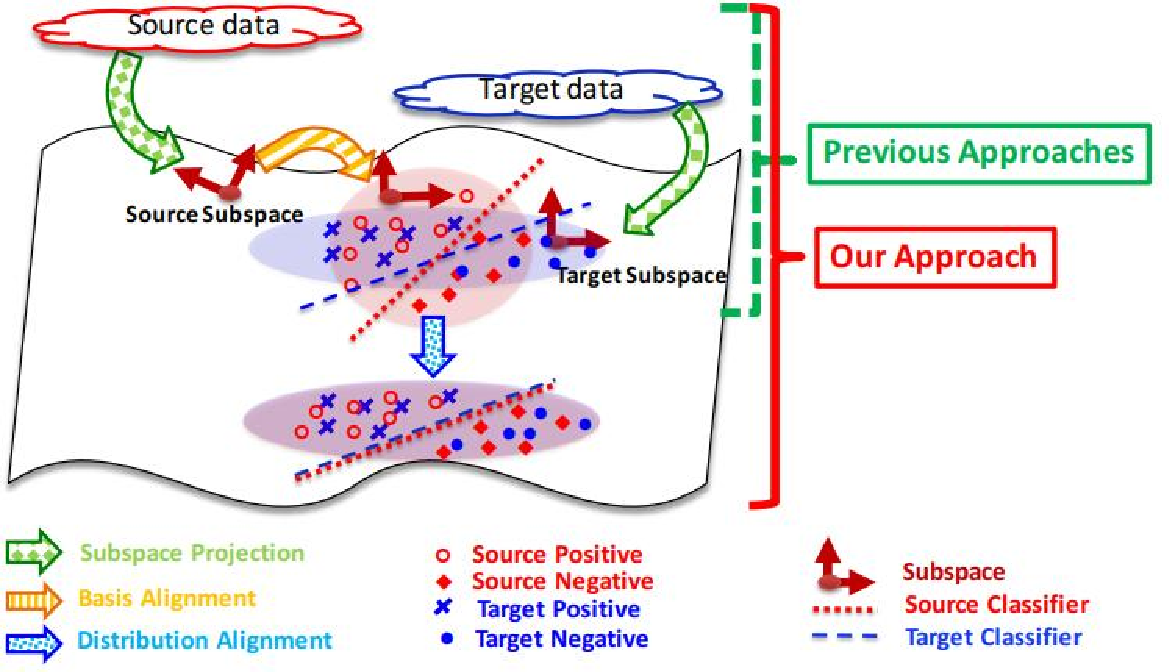
\includegraphics[scale=0.6]{./figures/fig-subspace-sda.pdf}
	\caption{SDA方法的示意图}
	\label{fig-subspace-sda}
\end{figure}

有别于SA和SDA方法只进行源域和目标域的一阶特征对齐,Sun等人提出了CORAL方法(CORrelation ALignment),对两个领域进行二阶特征对齐。假设$\mathbf{C}_s$和$\mathbf{C}_t$分别是源领域和目标领域的协方差矩阵,则CORAL方法学习一个二阶特征变换$\mathbf{A}$,使得源域和目标域的特征距离最小:

\begin{equation}
	\min_\mathbf{A} ||\mathbf{A}^\top \mathbf{C}_s \mathbf{A} - \mathbf{C}_t||^2_F
\end{equation}

CORAL方法的求解同样非常简单且高效。CORAL方法被应用到神经网络中,提出了DeepCORAL方法~\cite{sun2016deep}。作者将CORAL度量作为一个神经网络的损失进行计算。图展示了DeepCORAL方法的网络结构。

\begin{figure}[htbp]
	\centering
	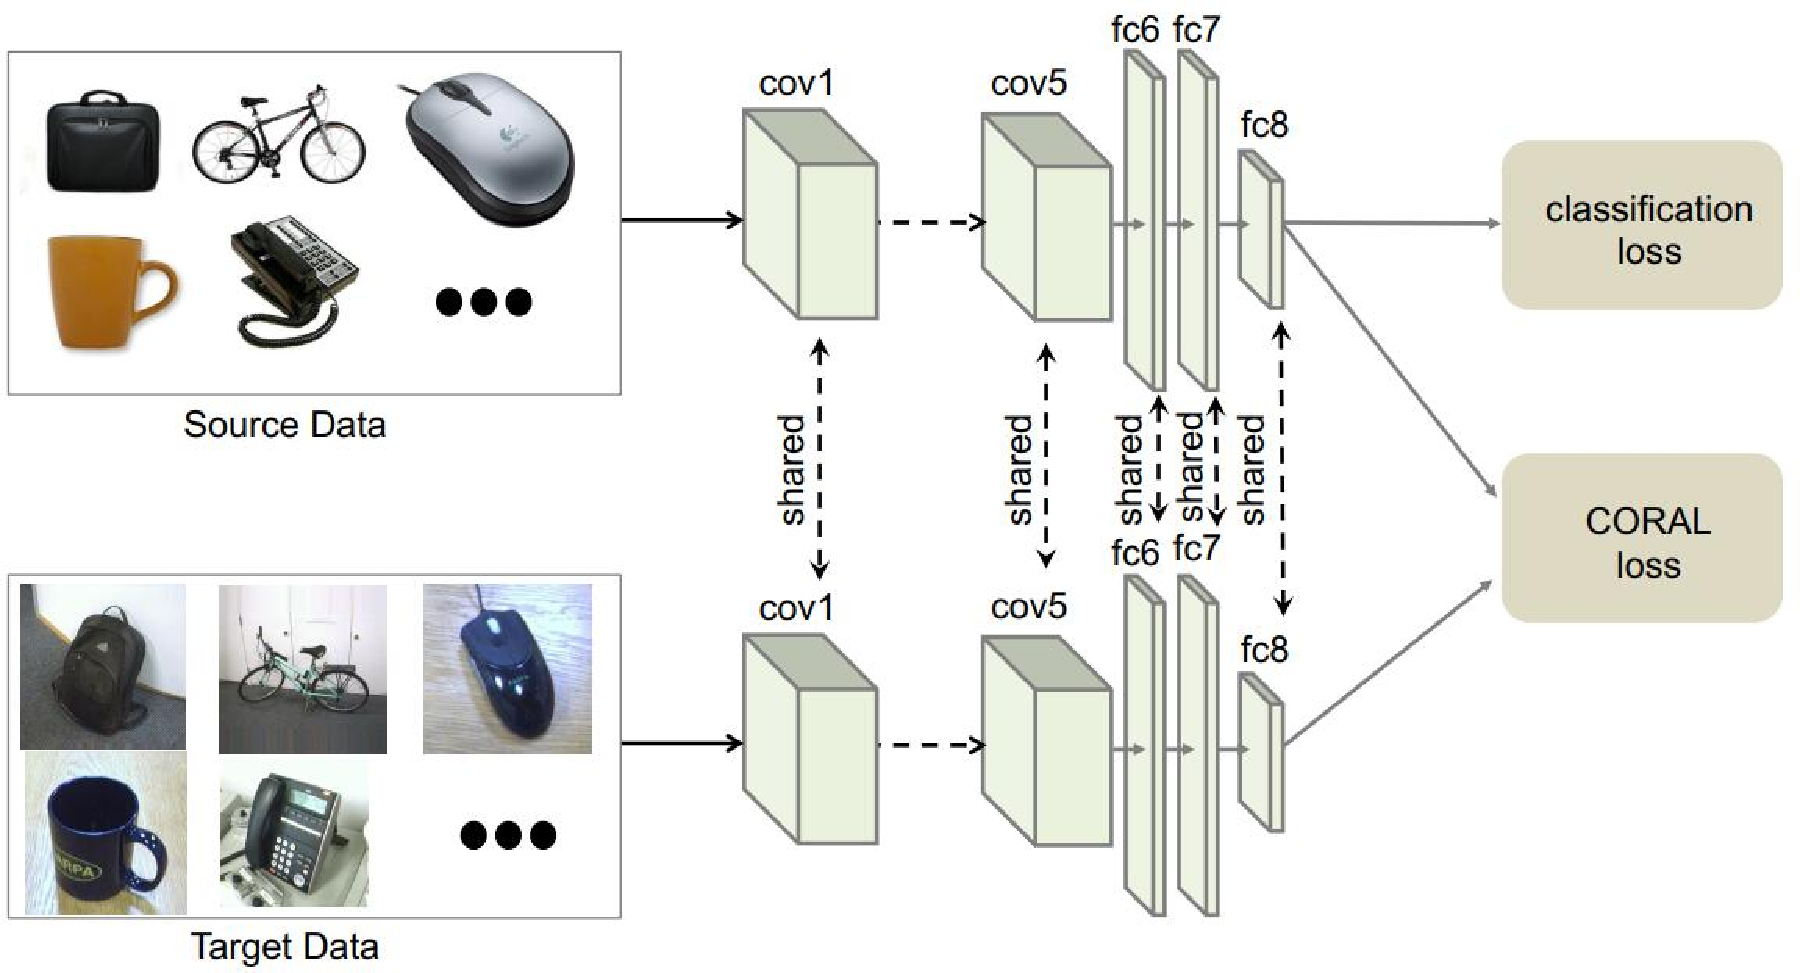
\includegraphics[scale=0.4]{./figures/fig-subspace-deepcoral.pdf}
	\caption{SDA方法的示意图}
	\label{fig-subspace-deepcoral}
\end{figure}

CORAL损失被定义为源域和目标域的二阶统计特征距离:

\begin{equation}
	\ell_{CORAL} = \frac{1}{4d^2} ||\mathbf{C}_s - \mathbf{C}_t||^2_F
\end{equation}

\subsection{流形学习}

流形学习自从2000年在Science上被提出来以后,就成为了机器学习和数据挖掘领域的热门问题。它的基本假设是,现有的数据是从一个\textit{高维空间}中采样出来的,所以,它具有高维空间中的低维流形结构。流形就是是一种几何对象(就是我们能想像能观测到的)。通俗点说就是,我们无法从原始的数据表达形式明显看出数据所具有的结构特征,那我把它想像成是处在一个高维空间,在这个高维空间里它是有个形状的。一个很好的例子就是星座。满天星星怎么描述?我们想像它们在一个更高维的宇宙空间里是有形状的,这就有了各自星座,比如织女座、猎户座。流形学习的经典方法有Isomap、locally linear embedding、laplacian eigenmap等。

流形空间中的距离度量:两点之间什么最短?在二维上是直线(线段),可在三维呢?地球上的两个点的最短距离可不是直线,它是把地球展开成二维平面后画的那条直线。那条线在三维的地球上就是一条曲线。这条曲线就表示了两个点之间的最短距离,我们叫它\textit{测地线}。更通俗一点,\textit{两点之间,测地线最短}。在流形学习中,我们遇到测量距离的时候,更多的时候用的就是这个测地线。在我们要介绍的GFK方法中,也是利用了这个测地线距离。比如在下面的图中,从A到C最短的距离在就是展开后的线段,但是在三维球体上看,它却是一条曲线。

\begin{figure}[htbp]
	\centering
	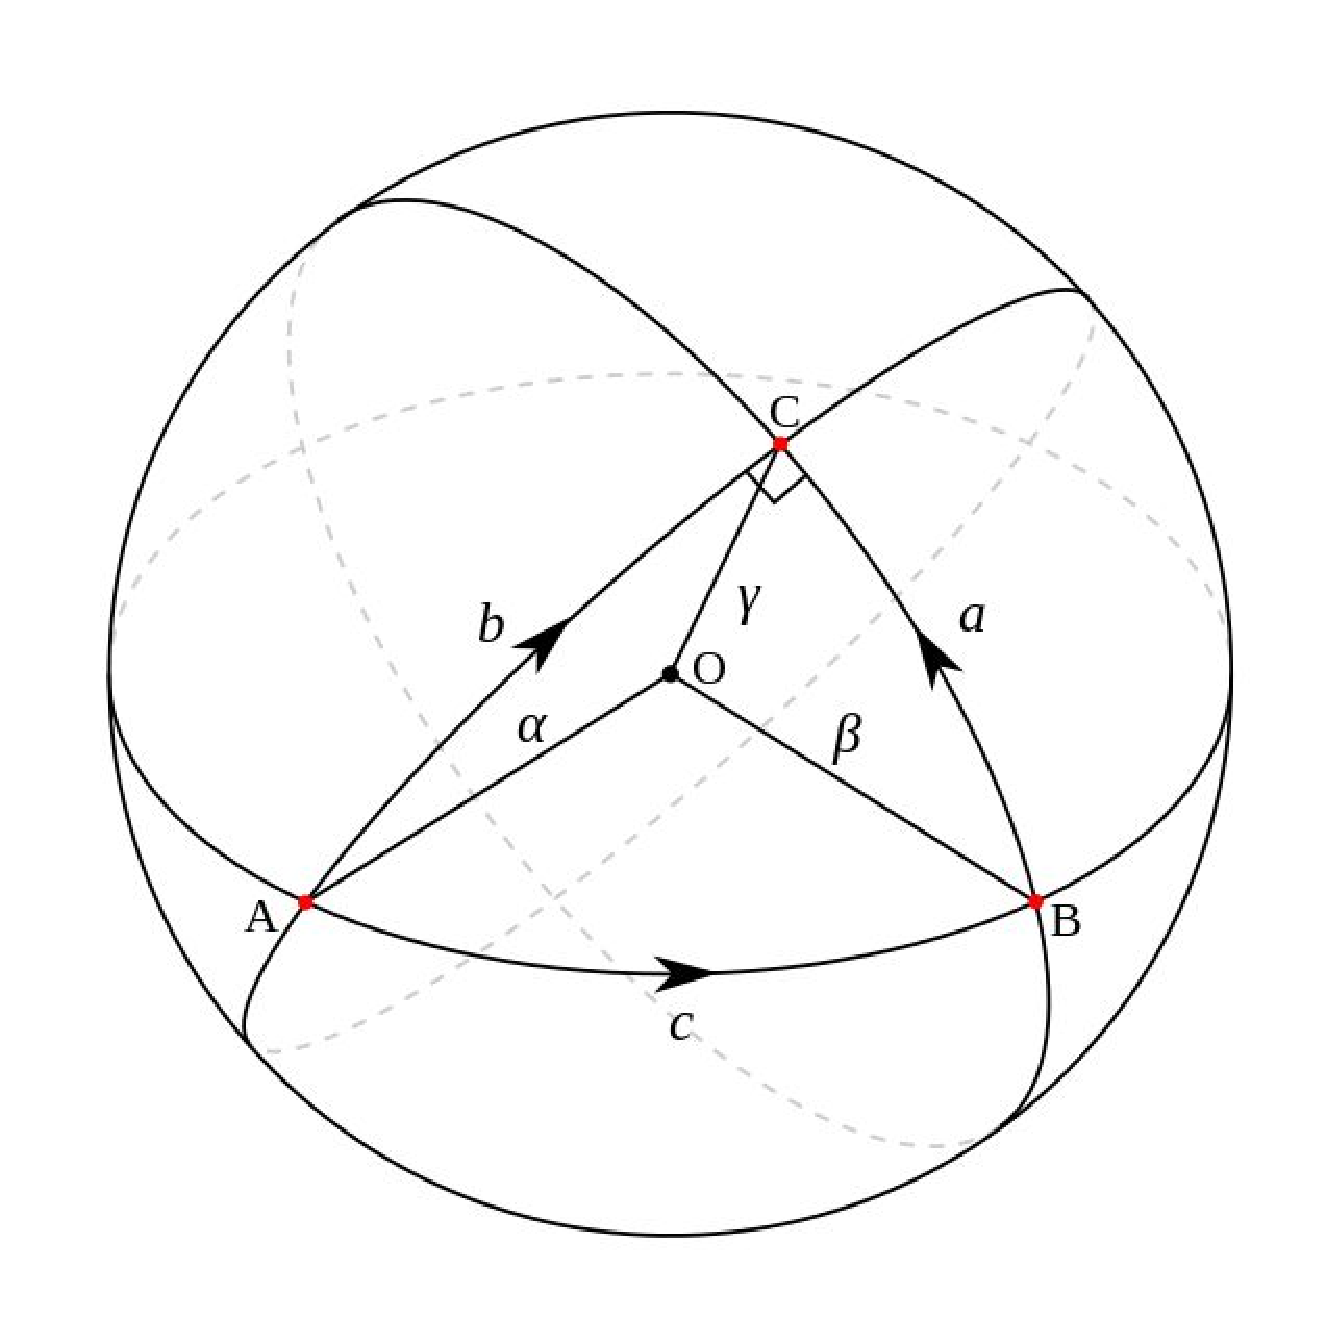
\includegraphics[scale=0.4]{./figures/fig-subspace-earth.pdf}
	\caption{三维空间中两点之间的距离示意图}
	\label{fig-subspace-earth}
\end{figure}

由于在流形空间中的特征通常都有着很好的几何性质,可以避免特征扭曲,因此我们首先将原始空间下的特征变换到流形空间中。在众多已知的流形中,Grassmann流形$\mathbb{G}(d)$可以通过将原始的$d$维子空间(特征向量)看作它基础的元素,从而可以帮助学习分类器。在Grassmann流形中,特征变换和分布适配通常都有着有效的数值形式,因此在迁移学习问题中可以被很高效地表示和求解~\cite{hamm2008grassmann}。因此,利用Grassmann流形空间中来进行迁移学习是可行的。现存有很多方法可以将原始特征变换到流形空间中~\cite{gopalan2011domain,baktashmotlagh2014domain}。

在众多的基于流形变换的迁移学习方法中,GFK(Geodesic Flow Kernel)方法~\cite{gong2012geodesic}是最为代表性的一个。GFK是在2011年发表在ICCV上的SGF方法~\cite{gopalan2011domain}发展起来的。我们首先介绍SGF方法。

SGF方法从\textit{增量学习}中得到启发:人类从一个点想到达另一个点,需要从这个点一步一步走到那一个点。那么,如果我们把源域和目标域都分别看成是高维空间中的两个点,由源域变换到目标域的过程不就完成了迁移学习吗?也就是说,\textit{路是一步一步走出来的}。

于是SGF就做了这个事情。它是怎么做的呢?把源域和目标域分别看成高维空间(即Grassmann流形)中的两个点,在这两个点的测地线距离上取$d$个中间点,然后依次连接起来。这样,源域和目标域就构成了一条测地线的路径。我们只需要找到合适的每一步的变换,就能从源域变换到目标域了。图~\ref{fig-subspace-sgf}是SGF方法的示意图。

\begin{figure}[htbp]
	\centering
	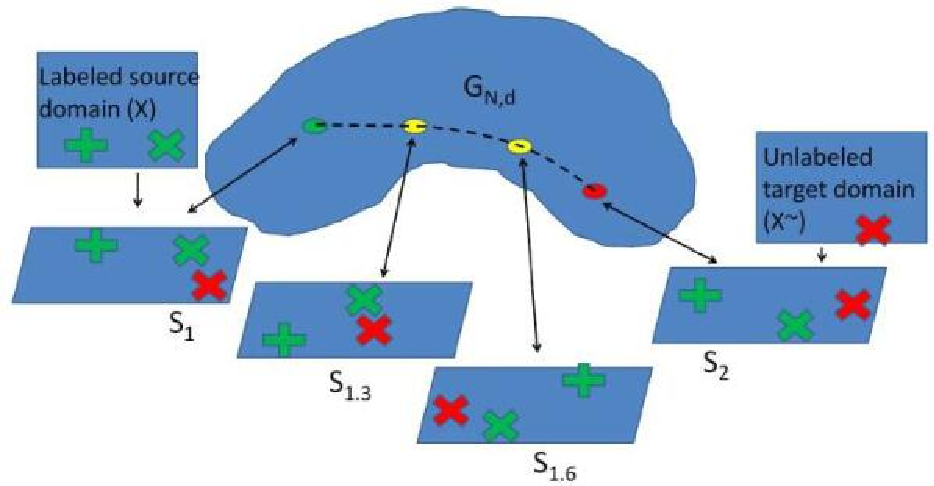
\includegraphics[scale=0.5]{./figures/fig-subspace-sgf.pdf}
	\caption{SGF流形迁移学习方法示意图}
	\label{fig-subspace-sgf}
\end{figure}

SGF方法的主要贡献在于:提出了这种变换的计算及实现了相应的算法。但是它有很明显的缺点:到底需要找几个中间点?SGF也没能给出答案,就是说这个参数$d$是没法估计的,没有一个好的方法。这个问题在GFK中被回答了。

GFK方法首先解决SGF的问题:如何确定中间点的个数$d$。它通过提出一种核学习的方法,利用路径上的无穷个点的\textit{积分},把这个问题解决了。这是第一个贡献。然后,它又解决了第二个问题:当有多个源域的时候,我们如何决定使用哪个源域跟目标域进行迁移?GFK通过提出Rank of Domain度量,度量出跟目标域最近的源域,来解决这个问题。图~\ref{fig-subspace-gfk}是GFK方法的示意图。

\begin{figure}[htbp]
	\centering
	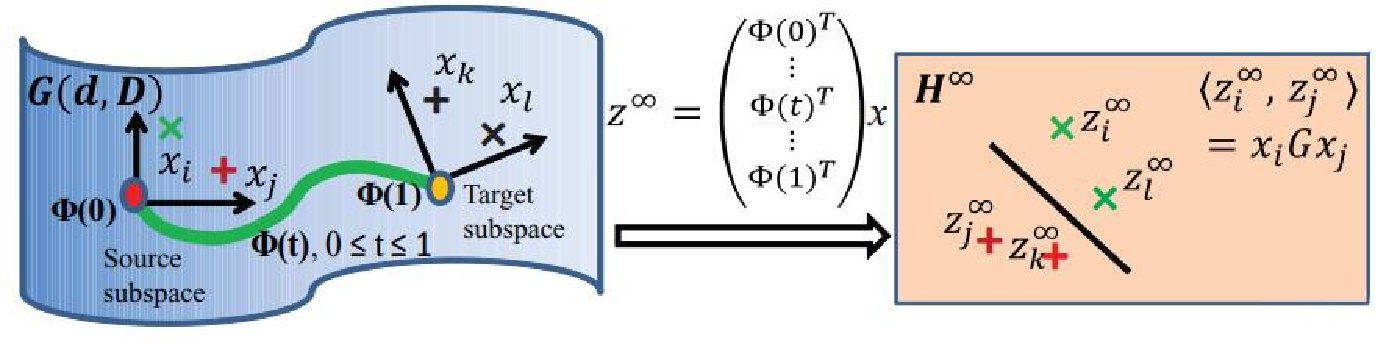
\includegraphics[scale=0.5]{./figures/fig-subspace-gfk.pdf}
	\caption{GFK流形迁移学习方法示意图}
	\label{fig-subspace-gfk}
\end{figure}

用$\mathcal{S}_s$和$\mathcal{S}_t$分别表示源域和目标域经过主成分分析(PCA)之后的子空间,则G可以视为所有的d维子空间的集合。每一个$d$维的原始子空间都可以被看作$\mathbb{G}$上的一个点。因此,在两点之间的测地线$\{\Phi(t):0 \leq t \leq 1\}$可以在两个子空间之间构成一条路径。如果我们令$\mathcal{S}_s=\Phi(0)$,$\mathcal{S}_t=\Phi(1)$,则寻找一条从$\Phi\left(0\right)$到$\Phi\left(1\right)$的测地线就等同于将原始的特征变换到一个无穷维度的空间中,最终减小域之间的漂移现象。这种方法可以被看作是一种从$\Phi\left(0\right)$到$\Phi\left(1\right)$的增量式“行走”方法。

特别地,流形空间中的特征可以被表示为$\mathbf{z}=\Phi\left(t\right)^\top \mathbf{x}$。变换后的特征$\mathbf{z}_i$和$\mathbf{z}_j$的内积定义了一个半正定(positive semidefinite)的测地线流式核
\begin{equation}
	\langle\mathbf{z}_i,\mathbf{z}_j\rangle= \int_{0}^{1} (\Phi(t)^T \mathbf{x}_i)^T (\Phi(t)^T \mathbf{x}_j) \, dt = \mathbf{x}^T_i \mathbf{G} \mathbf{x}_j
\end{equation}

GFK方法详细的计算过程可以参考原始的文章,我们在这里不再赘述。

\subsection{扩展与小结}

子空间学习方法和概率分布自适应方法可以有机地进行组合,克服各自的缺点。下面是一些相关工作。

\begin{itemize}
	\item DIP (Domain-Invariant Projection)~\cite{baktashmotlagh2013unsupervised}: 边缘分布自适应+流形变换
	\item \cite{baktashmotlagh2014domain}: 统计流形法,在黎曼流形上进行距离度量。
\end{itemize}

最近的一些工作~\cite{sun2016deep}显示,子空间学习法和神经网络的结合会更好。
